%Basic Formatting and Packages---------------------------------------------------------------------------------------------------------------------------------------------------------------------------
\documentclass[11pt,a4paper]{article}
\usepackage{amsmath} 
\usepackage{amssymb}   
\usepackage{graphicx}
\usepackage{geometry}
\usepackage{mathtools}
\usepackage[dvipsnames]{xcolor}
\usepackage{enumitem}
\usepackage{tcolorbox}
\usepackage{verbatim}
\usepackage{subcaption}
\usepackage[ruled, noend]{algorithm2e}

\usepackage{tikz}
\usetikzlibrary{shapes.geometric, arrows, positioning}

\geometry{left=2cm,right=2cm,top=2.5cm,bottom=2.5cm}


%Own Commands----------------------------------------------------------------------------------------------------------------------------------------------------------------------------------------------------
%1. Inequality in set: ieset
%Default: lhs is tau
\newcommand{\ieset}[2][\tau]{\{#1 \le #2\}} 
%Example: to get {X <= t} use this expression $\ieset[X]{t}$

%2. Conditional Expectation for Sigma Algebra: scEx
%Default: sigma Algebra is F_n
\newcommand{\scEx}[2][n]{E[#2 \mid \mathfrak{F}_#1]}
%Example: to get E[ X | F_tau ] use this expression $\scEx[\tau]{X}$

%3. In curly brackets: icb
\newcommand{\icb}[1]{\{ #1 \}}
%Example: to get {a = b} use this expression $\icb{a = b}

%4. Norm: norm
\newcommand{\norm}[1]{\left\lVert#1\right\rVert}
%Example: to get ||X|| use the expression \norm{X}

%5. Column Vector
\newcommand*\colvec[1]{\begin{pmatrix}#1\end{pmatrix}}
%Example: \colvec{a \\ b} gives vector (a,b) transposed.

%6.Row Vector
\newcommand{\rvec}[1]{\begin{bmatrix} #1 \end{bmatrix}}
%Example: \rvect{a & b} gives vector (a,b)


%Own Operators----------------------------------------------------------------------------------------------------------------------------------------------------------------------------------------------------
\DeclareMathOperator*{\argmax}{arg\,max}
\DeclareMathOperator*{\argmin}{arg\,min}




\title{Collection}

\begin{document}

%Inputs from content----------------------------------------------------------------------------------------------------------------------------------------------------------------------------------------------------
\section{The harm of class imbalance corrections for risk prediction models}
	The paper argues that the class imbalance is not a pervasive problem for prediction model development. 
	First, the problem is specific to the classification accuracy measure. 
	The limitations of focusing on classification accuracy as a measure of predictive performance is well known. 
	Second, if we consider models that produce estimated probabilities of the event of interest, 
	an adjustment of the classification threshold probability can be used to ensure adequate classification performance 
	(ie, probability threshold to classify individuals as high risk does not have to be 0.5). 
	A probability threshold to select individuals for a given treatment implies certain misclassification costs and should be determined using clinical considerations. 
	If we use a probability threshold of 0.1 to classify individuals as high risk and suggest a specific treatment, 
	this means that we accept to treat up to 10 individuals in order to treat 1 individual with the event: 
	we accept up to 9 false positives, or unnecessary treatments, per true positive.
	
\subsection{Discussion}
	\begin{figure}[h]
         	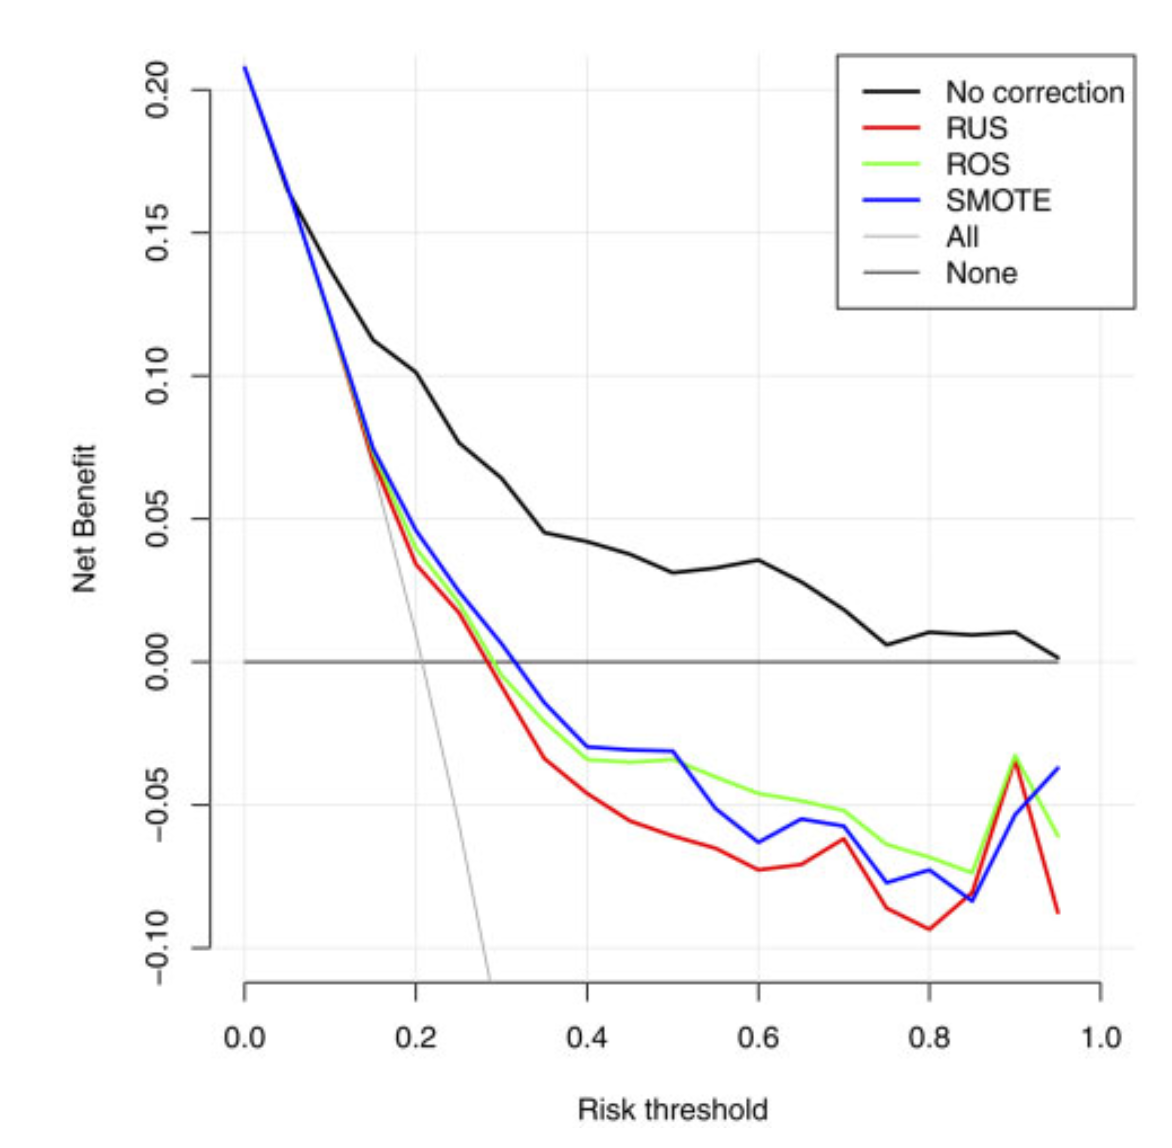
\includegraphics[height=0.5\textheight]{assets/harm_class_imbalance_corr/risk_benefit_SMOTE_RUS_ROS.png}
         	\caption{Risk vs Net Benefit for uncorrected vs ROS, RUS and SMOTE}
         \end{figure}
	The key finding of our work is that training logistic regression models on imbalance corrected data did not lead to better AUROC 
	compared to models trained on uncorrected data, but did result in strong and systematic overestimation of the probability for the minority class. 
	In addition, all imbalance corrections had negative consequences for the calibration slope. 
	The lower the event fraction, the more outspoken the results.
	
	Strong miscalibration reduces the clinical utility of a prediction model.30 Models yielding probability estimates that are clearly too high may lead to overtreatment. 
	For example, if a model overestimates the risk of malignancy of a detected ovarian tumor, the decision to refer patients to specialized surgery may be taken too quickly. 
	Class imbalance is often framed as problematic in the context of prediction models that classify patients into low-risk versus high-risk groups. 
	Nevertheless, for clinical prediction models the accurate estimation of probabilities is essential to help in defining such low-risk and high-risk groups. 
	For instance, clinical staff using the model to support treatment decisions may choose probability thresholds
	to match the assumed misclassification costs that best fit the context.
	
	In contrast, our study suggests that, at least for logistic regression models, 
	RUS (or ROS or SMOTE) is unlikely to lead to better discrimination or separability between the minority and majority classes.
	
\subsection{Conclusion}	
	Our study shows that correcting class imbalance did not result in better prediction models based on standard or ridge logistic regression. 
	The imbalance corrections resulted in inaccurate probability estimates without improving discrimination in terms of AUROC.
	
	

\section{Metrics}
<<<<<<< HEAD
\subsection{Accuracy rate}

	If benefit and harm are weighted equally, the odds of the threshold is 1:1, or a threshold probability of $50\%$. 
	This cutoff is by default considered in the calculation of the error rate, which is defined as (FN + FP)/N. 
	The complement is the accuracy rate: (TN + TP)/N.
	Often FN classifications are more important than FP classifications, which makes the accuracy rate not a sensible indicator of clinical usefulness.
	Other disadvantages include that the accuracy rate by definition is high for a frequent or infrequent outcome (i.e. imbalanced data).
	
	The accuracy rate is usually calculated at the simplistic cutoff of $50\%$, but can also be calculated at clinically defendable thresholds. 
	The harm-to-benefit ratio that underpins the choice of the cutoff should then be used to calculate a weighted accuracy, or its complement, the weighted error rate.
	We can express the TN classifications in units of the TP classifications, such that the weighted accuracy is calculated as (TP + w TN)/n.
	
	The improvement that is obtained by making decisions based on predictions from the model is the difference between the weighted accuracy
	obtained with the model versus the weighted accuracy of the default policy.
	
=======

>>>>>>> baseline
\subsection{Receiver Operator Characteristic (ROC)}
	Consider a binary classification problem where we have a classifier that outputs a continuous score s(X) for an instance X.
	We then set a threshold $\tau$ to decide the predicted class. If $s(X) > \tau$, we predict the positive class; otherwise, we predict the negative class.
	
    	\begin{align*}
    		TPR(\tau) &= \mathbb{P}(s(X) > \tau | Y = 1) \\
    		FPR(\tau) &= \mathbb{P}(s(X) > \tau | Y = 0)
    	\end{align*}
	
	Here, $Y$ is the true class of an instance. 
	TPR is the probability that the classifier ranks a randomly chosen positive instance higher than a randomly chosen negative instance. 
	Similarly, FPR is the probability that the classifier ranks a randomly chosen negative instance higher than a randomly chosen positive instance.
    
    	
	The ROC curve plots $TPR(\tau)$ against $FPR(\tau)$ for all possible thresholds $\tau$, producing a curve that ranges from $(0,0)$ to $(1,1)$.
	We can interpret a ROC plot as plotting the path of a function
	\[
		f: \mathbb{R} \to [0,1]^2, \quad  \tau \mapsto (TPR(\tau), FPR(\tau))
	\]
	The Area Under the ROC Curve (AUC) then provides a single scalar value that represents the expected performance of the classifier.
	An AUC of $1$ indicates a perfect classifier, while an AUC of $0.5$ indicates a classifier that performs no better than random chance.
	
	AUC can also be interpreted in terms of the probability that the classifier will rank a randomly chosen positive instance higher than a randomly chosen negative instance,
	assuming that one positive and one negative instance are chosen at random.
<<<<<<< HEAD
	The area under the curve (AUC) can be interpreted as the probability that a patient with the outcome is given a higher probability of the outcome by the model
	than a randomly chosen patient without the outcome
	Some may consider the interpretation of AUC as straightforward. Others may object that we consider a pair of subjects, one with and one without the outcome, 
	and that such conditioning is a rather artificial situation. 
	Statistically, this conditioning on a pair of patients is attractive, since it makes the area independent of the incidence of the outcome (or event rate), 
	in contrast to R2 or the Brier score, for example.
	The AUC is a rank order statistic.
	As a rank order statistic, it is insensitive to errors in calibration such as differences in average outcome.
	Confidence intervals for the AUC (or c statistic) can be calculated with various methods. 
	Standard asymptotic methods may be problematic, especially when sensitivity or specificity is close to $0\%$ or $100\%$. 
	Bootstrap resampling is a good choice for many situations.
	
	
	
\subsection{Net Benefit}
	The choice of risk threshold implicitly conveys the adopted relative misclassification costs. 
	It can be derived that the odds of the risk threshold equal the harm-to-benefit ratio, which is the harm of a false positive divided by the benefit of a true positive.
	For example, if a risk threshold of $20\%$ is used, the odds are 1 to 4. 
	Therefore, a $20\%$ risk threshold assumes that the harm of a false positive is one-quarter of the benefit of a true positive or that 1 true positive is worth 4 false positives: 
	A clinician might express this in terms such as ‘‘I would not do more than five biopsies to find one cancer.’’ 
	Hence, when applying a model to a set of patients,
	we can correct the number of true positives (TP) for the number of false positive (FP) using the odds $w$ of the risk threshold $t$: 
	\[
		\text{TP} - w \text{FP} = \text{TP} - \frac{\tau}{1-\tau} \text{FP}
	\]
	When dividing by the total sample size $N$, the Net Benefit is obtained
	\[
		\text{NB} = \frac{1}{N} (\text{TP} - w \text{FP}) = \frac{1}{N} (\text{TP} - \frac{\tau}{1-\tau} \text{FP})
	\]
	
	The Net Benefit of treat-none is always 0, 
	whereas the Net Benefit of treat-all is positive for risk thresholds below the event rate and negative for risk thresholds above the event rate.
	
	%Note that the mis- calibration induced by changing either the intercept or the slope does not affect AUC because the rank order of risks is not changed.
	
\subsection{Net Benefit and Risk Threshold}
	Suppose r.v. $Y$ with outcome diseased $D$ or healthy $\neg D$.
	Let $c_{TP}, c_{FP}, c_{TN}, c_{FN}$ then expected cost of predicting $\neg D$ is
	\[
		\mathbb{P}(Y = 1) c_{FN} + \mathbb{P}(Y = 0) c_{TN}
	\]
	
	and expected cost for predicting $D$ is
	\[
		\mathbb{P}(Y = 1) c_{TP} + \mathbb{P}(Y = 0) c_{FP}
	\]
	
	If we write $T = \mathbb{P}(Y = 1)$ we can rewrite to
	\[
		T c_{FN} + (1-T) c_{TN}
	\]
	and
	\[
		T c_{TP} + (1-T) c_{FP}
	\]
	One is indifferent about treatment if both expected costs are equal.
	\[
	\begin{aligned}
		T c_{FN} + (1-T) c_{TN} &= T c_{TP} + (1-T) c_{FP} \\
		&\Leftrightarrow \\
		T &= \frac{c_{TN} - c_{FP}}{(c_{TN} - c_{FP}) + (c_{TP} - c_{FN})} \\
	\end{aligned}
	\]
	It can also be rearranged in a different way
	\[
	\begin{aligned}
		T c_{FN} + (1-T) c_{TN} &= T c_{TP} + (1-T) c_{FP} \\
		&\Leftrightarrow \\
		\frac{T}{1 - T} &= \frac{ c_{TN} - c_{FP} }{ c_{TP} - c_{FN} } \\
	\end{aligned}
	\]
	
	In the first group, the costs relate to undertreatment (false-negative classifications)
	The costs of these false-negative classifications $c_{FN}$ should be compared to the costs of true-positive classifications $c_{TP}$.
	The difference $c_{TP} - c_{FN}$ is the net benefit of treating all who have the disease compared to treating none of them.
	Suppose you have a treatment that causes lots of damage as well as curing the disease. 
	Then this difference might be low, i.e. treating everyone with the dangerous treatment does not give much better outcome than simply not treating anyone.
	Suppose on the other hand you have a devastating disease like Polio and a low cost treatment like a Polio-vaccine, then that difference will be strongly positive.
	
	In the second group, relevant costs are for those without the event if not treated, who are treated (“overtreated”).
	The costs of these false-positive classifications ($c_{FP}$) should be compared to the costs of true-negative classifications ($c_{TN}$)
	while $c_{TN} - c_{FP}$ is the harm of treating all who don't have the disease compared to the benefit of not treating any of them.
	E.g. the cost of not treating anyone without the disease might be 0 but the cost of treating them might be high. Then this value is strongly negative.
	On the other hand suppose again a low impact vaccine that barely does harm, then that difference may be small negative. 
	
	Odds (cutoff) = Harm/Benefit
	
	The ratio in case of e.g. the polio vaccine could be strongly in favour of treating everyone (small cost for those without, high benefit for those with disease).
	
	
	
\subsection{Calibration}
	Another key property of a prediction model is calibration, i.e., the agreement between observed outcomes and predictions.
	\[
		TPR(\tau) = \mathbb{P}(s(X) > \tau | Y = 1)
	\]


\subsection{Mixed}
	\begin{align*}
    		\color{teal} TPR(\tau) &= \mathbb{P}(s(X) > \tau | Y = 1) \\
    		\color{purple} FPR(\tau) &= \mathbb{P}(s(X) > \tau | Y = 0) \\
    	\end{align*}

	
=======
	




>>>>>>> baseline






	
\end{document}